

To deploy LTE-U base stations in public,
it is important to make it Wi-Fi friendly.  
We propose to use CTS-to-self to notify Wi-Fi APs the existence
of LTE-U. 
As we discuss in previous section, medium utilization is not sufficient
to estimate channel utilization since different 
versions of Wi-Fi networks, 802.11a/b/g/m, 
shows different level of medium utilization. 
Instead of looking at the MU of a monitoring interval, 
we look at the change of MU ($\Delta{MU}$) in two continuous monitoring intervals. 
The basic obervation is, the $\Delta{MU}$ of saturated link is smaller
than that of unsaturated link. 


\subsection{Pre-Encoding CTS-to-self}


\begin{figure}[!ht]
 \centering
    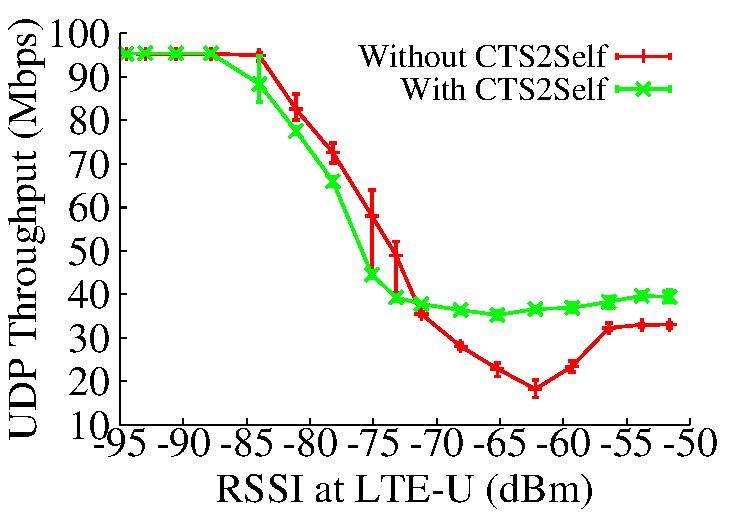
\includegraphics[width=2.6in]{./figures/cts2self_power}
 \caption{CTS-to-self.}
  \label{fig:cts2self_power}
\end{figure}

Using CTS-to-self to coexist with Wi-Fi networks is not a novel idea. 
Different Wi-Fi versions use CTS as a mechanism to reserve 
wireless channels. 
This is because 802.11b/g routers are not able to detect
802.11n packets due to different modulations, 
newer Wi-Fi version uses same coexist techniques to 
reserve channel. 
Since we use software defined radio, encoding CTS
in real time is challenging, 
as we need to encode how many subframes (or milliseconds) the LTE-U wants
to reserve. 
Therefore, we encode the Wi-Fi preamble and CTS in the physical layer. 
The CTS-to-self is evaluated by using TP-Link router
and the results are shown in Fig. \ref{fig:cts2self_power}.
If all the Wi-Fi routers are using the sensing and 
rate adaptation algorithm implemented in OpenWRT, 
CTS-to-self may be not required for coexistence. 
CTS-to-self adds extra overhead to LTE-U transmissions,
i.e., Wi-Fi preamble and CTS frame etc. 



\subsection{Reactive Adaptation}

The key observation we make from the previous experiments is that it is difficult to set a common medium utilization threshold for all scenarios. However, we also observe that if the medium is not fully saturated, the medium utilization of Wi-Fi keeps increasing as the LTE-U duty cycle increases (as shown in the examples in Figure~\ref{fig:csat_mu_good}). Once the medium is saturated, this is not true any more (as shown in the examples in Figure~\ref{fig:csat_mu_bad}). 



\begin{figure}[tbp]
\centering
\begin{minipage}{.45\textwidth}
  \centering
\begin{algorithmic}[1]
 {\small
  \Function{RAT}{$t$} 

        \State $\Delta_{MU} = \overline{MU}(t) - \overline{MU}(t-T)$
        \State $\Delta_{on} = {ON}_{mss}(t) - {ON}_{mss}(t-T)$
        \State $\beta = curmu * mu_{\alpha}$;
 
        \State $T_{UP} = \min ( T_{ON}(n) + \Delta T_{UP}, T^{max}_{ON})$;
        \State $T_{DOWN} = \min ( T_{ON}(n) - \Delta T_{DN}, T^{min}_{ON})$;

        \If { $\Delta_{on} > 0$}            \label{rat:ups}
          \If { $\Delta_{MU} > \beta$ }
            \State $T_{ON}(n+1) = T_{UP}$;
          \ElsIf {$\Delta_{MU} < -\beta$}   \label{rat:upd}
            \State $T_{ON}(n+1) = T_{DOWN}$;
          \Else
            \State $T_{ON}(n+1) = T_{DOWN}$;
          \EndIf                           \label{rat:upe}
       \ElsIf { $\Delta_{on} == 0$} 
          \If {$\Delta_{MU} > \beta$}        \label{rat:eqs}
            \State $T_{ON}(n+1) = T_{UP}$;
          \ElsIf {$\Delta_{MU} < -\beta$}    \label{rat:eqd}
            \State $T_{ON}(n+1) = T_{DOWN}$;
          \Else
            \State $T_{ON}(n+1) = T_{ON}(n)$;
          \EndIf                            \label{rat:eqe}
       \Else                                \label{rat:dns}
          \If {$\Delta_{MU} > \beta$}
            \State $T_{ON}(n+1) = T_{DOWN}$;
          \ElsIf {$\Delta_{MU} < -\beta$}
            \State $T_{ON}(n+1) = T_{UP}$;
          \Else
            \State $T_{ON}(n+1) = T_{DOWN}$;
          \EndIf                            \label{rat:dne}
       \EndIf
	
	
\EndFunction
}
%\Statex
\end{algorithmic}
\end{minipage}
\caption{{Reactive adaptation (RAT).}} 
\label{fig:rat}
\vspace{-6pt}
\end{figure}

Based on these observation, we propose a different duty cycle adaptation algorithm we call {\em Reactive adaptation} (RAT), described in Figure~\ref{fig:rat}. 
RAT tries to infer Wi-Fi flow saturation by observing the medium utilization change as a reaction to the duty cycle changing. 
RAT probes the medium by slightly increasing or decreasing the LTE-U load, using the same increments as CSAT. 
After each probe RAT measures the relative change in medium utilization. 
In case we increased the duty cycle and at the same the medium utilization increased by more than a threshold $\beta$ (lines \ref{rat:ups}-\ref{rat:upd}), this means that there is more scope for a utilization increase and we keep increasing the duty cycle. 
However, if no significant medium utilization increase has been observed (less than $\beta$, lines \ref{rat:upd}-\ref{rat:upe}), we conclude that the medium is already saturated and we decrease the duty cycle. 
We deal with a decrease in the duty cycle in a similar manner (lines \ref{rat:dns}-\ref{rat:dne}). 

If the duty cycle hasn't previously changed (because it has already reached the limit), then in the next step we change the duty cycle the same way the utilization has changed. 
If the utilization has gone up (lines \ref{rat:eqs}-\ref{rat:eqd}), this implies that there may be more scope for traffic increase and we increase the duty cycle. Otherwise we conservatively decrease it (lines \ref{rat:eqd}-\ref{rat:eqe}).

The threshold $\beta$ is calculated from the last medium utilization $MU(n)$. We determine the multiplicative factor $mu_{\alpha}$ by experimenting in various networks. We find that the best value is $mu_{\alpha} = 0.15$.

We illustrate the effects of RAT on the hidden node topology shown in Figure~\ref{fig:csat_hidden}. 
We plot the throughput achieved by AP 1 in Figure~\ref{fig:csat_mu_bad}, right. 
We see that in this example the Wi-Fi AP 1 achieves much higher throughput when LTE-U node runs RAT, and is never starved. 
We further quantify the benefits of RAT in real-world scenarios in Section~\ref{sec:eval}.

As a conclusion, we see that LTE-U duty-cycle adaptation should not be based on the average medium utilization, as the metric is too simplistic. Instead, one should adapt the duty-cycle based on the effects its changes have on the network traffic, as proposed in RAT.
 

%% \subsection{Extended Fairness Definition}
%% %\subsection{LTE-U's Fair Share}

%% The advance CSAT achieves the same share as backlogged Wi-Fi in a single collision domain,
%% and achieves better fairness (for example, using max-min fairness) than backlogged Wi-Fi in exposed terminal case.

%% \input{./doc/fairshare.tex}


%% %How to evaluate:
%% %compare the converged states in controlled environment: (1) LTE-U (2) a full backlogged Wi-Fi.







